\begin{frame}
\frametitle{Learning network protocols despite mismatched assumptions}
\begin{centering}
Can we learn a protocol that performs well both when there are few senders and when there are many senders?
\end{centering}
\end{frame}

\begin{frame}
\frametitle{Imperfections in the number of senders}
\begin{centering}

\noindent \only<1>{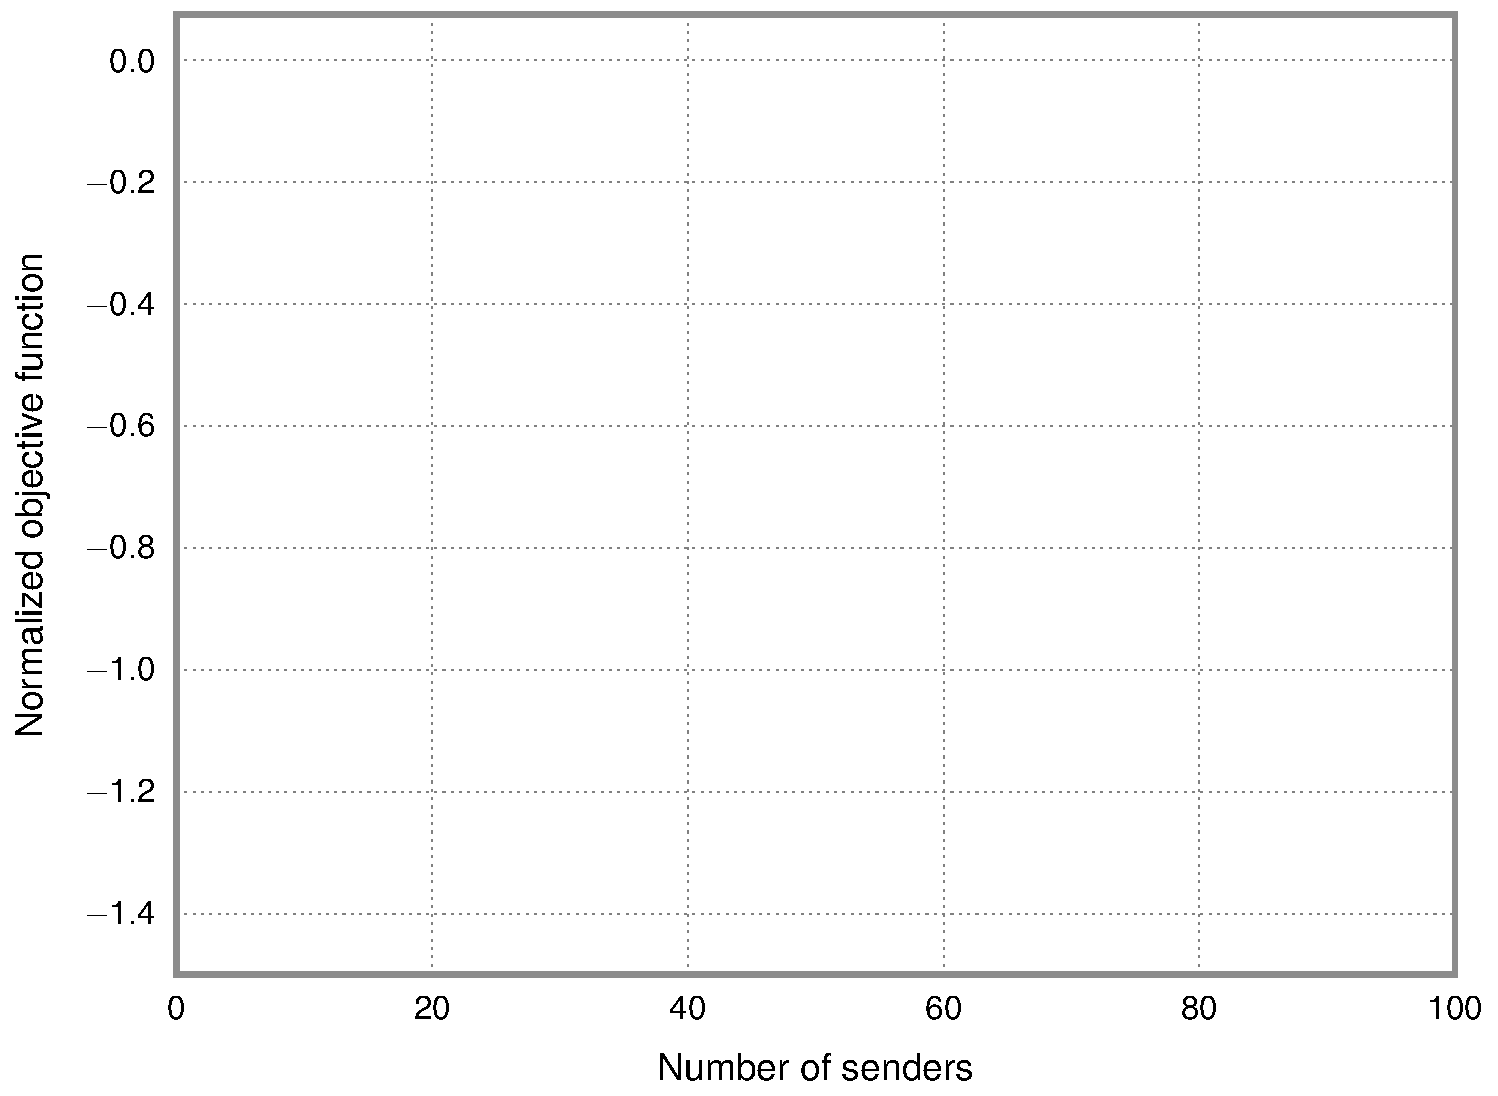
\includegraphics[width=4.1 in]{muxing-base.pdf}}\only<2>{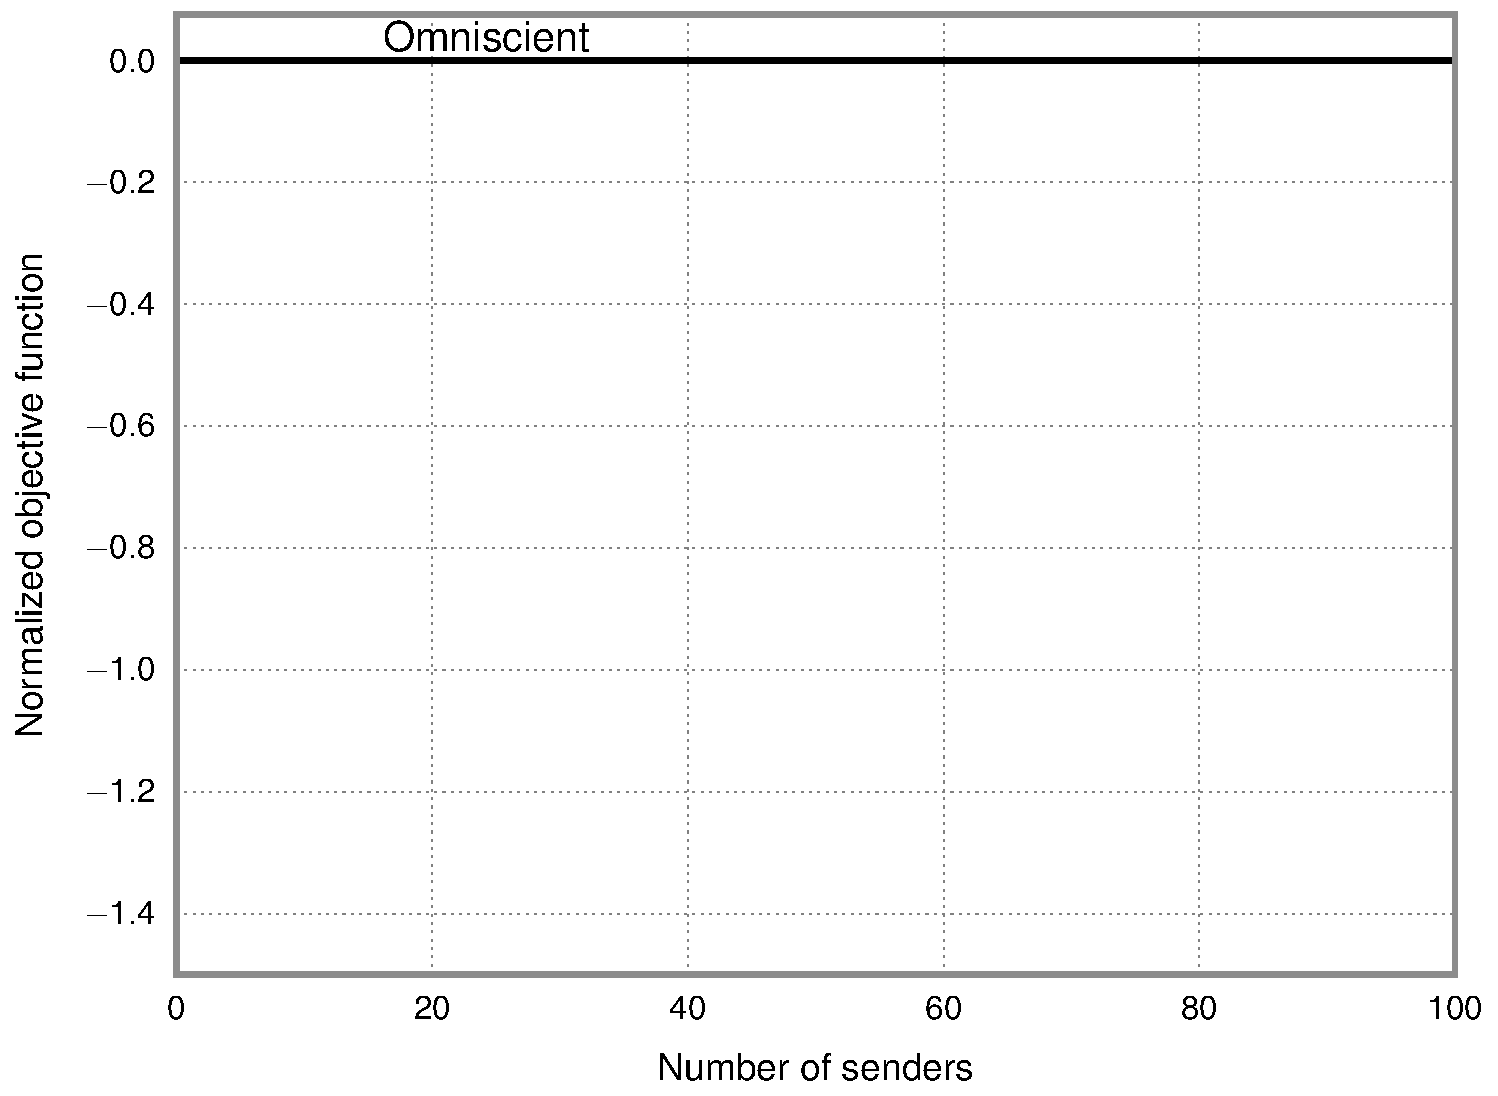
\includegraphics[width=4.1 in]{muxing-omniscient.pdf}}\only<3>{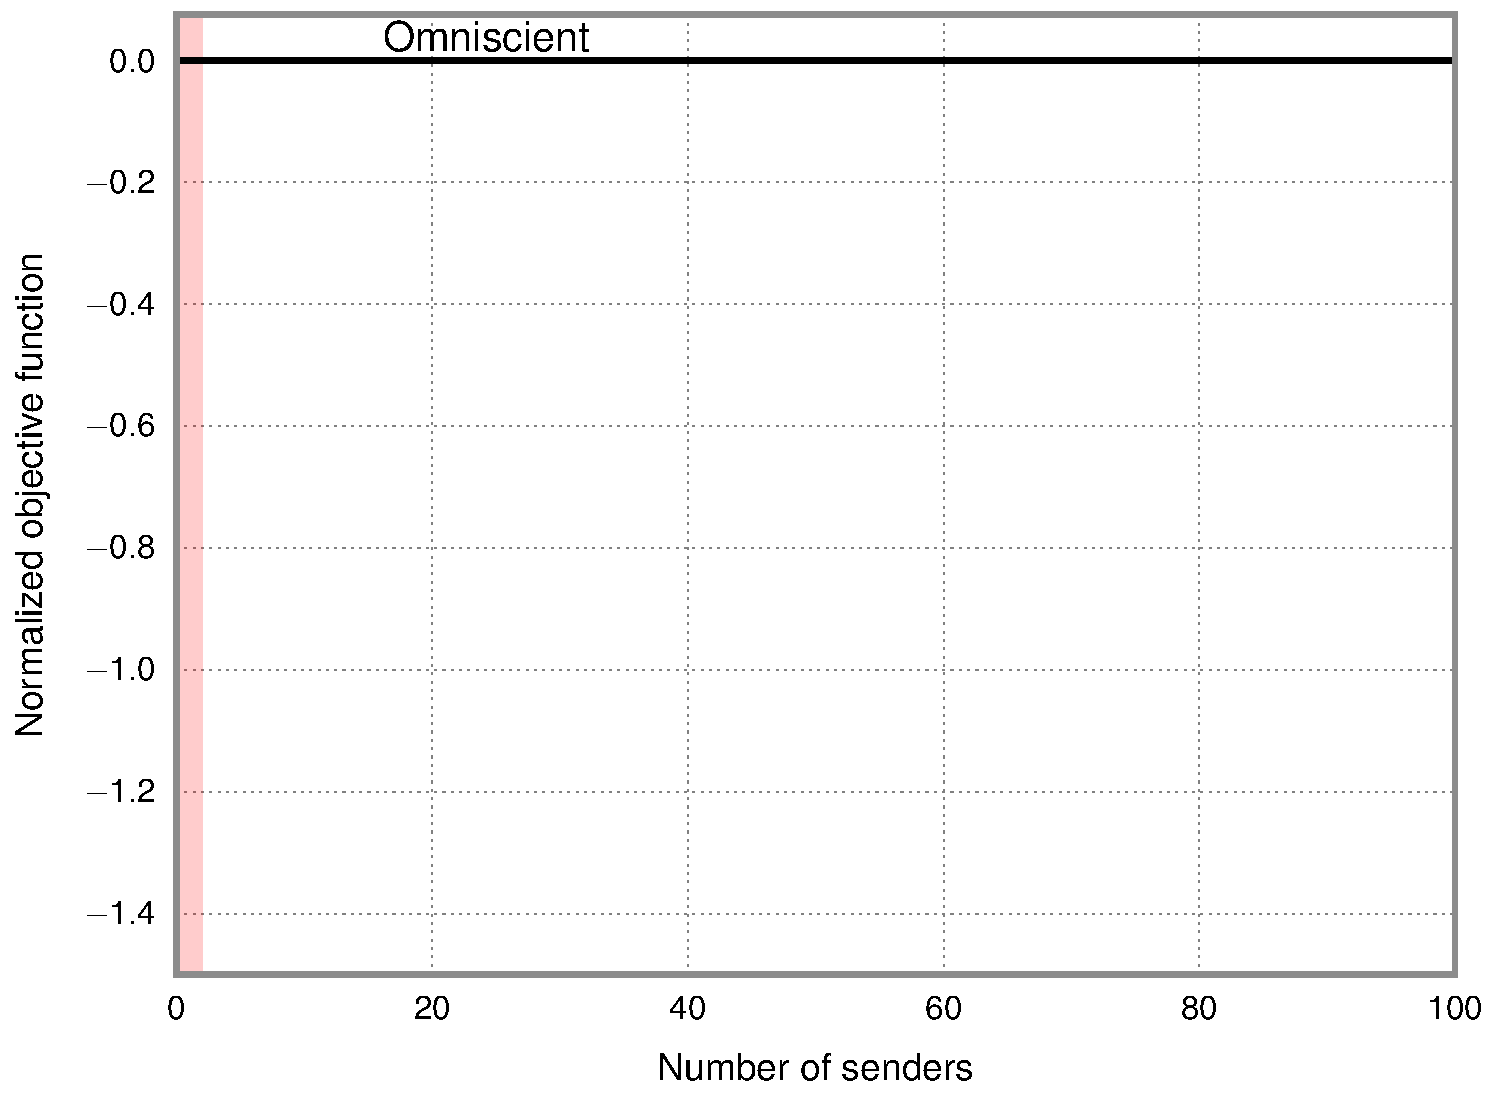
\includegraphics[width=4.1 in]{muxing-span-Tao-1-2.pdf}}\only<4>{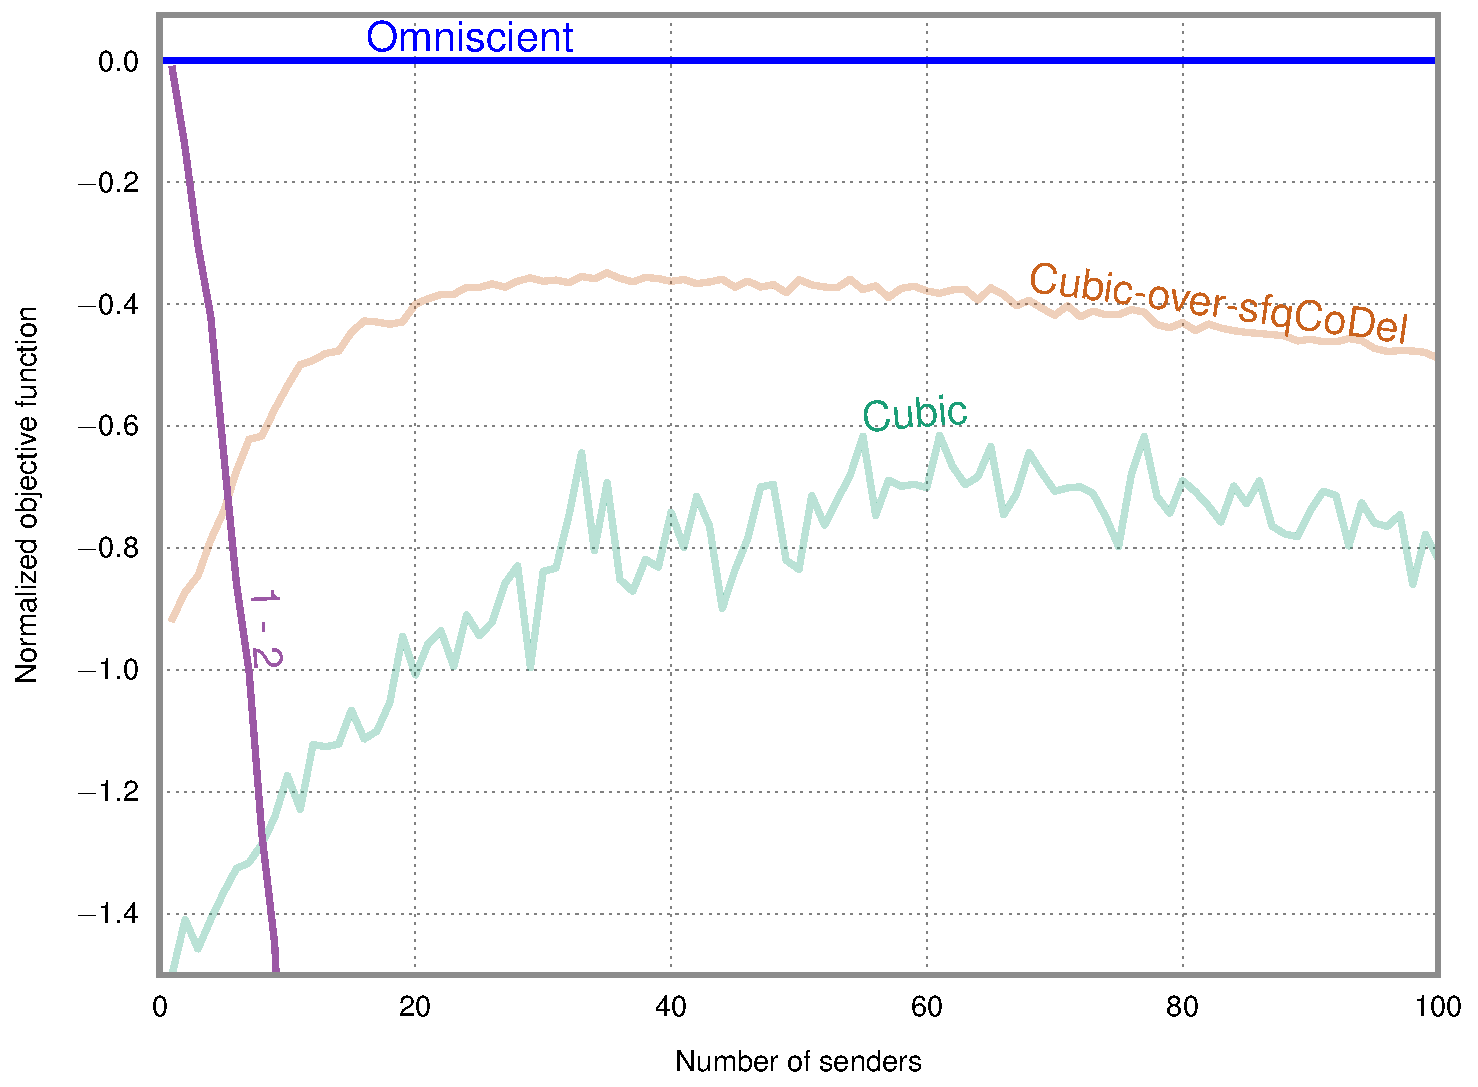
\includegraphics[width=4.1 in]{muxing-Tao-1-2.pdf}}\only<5>{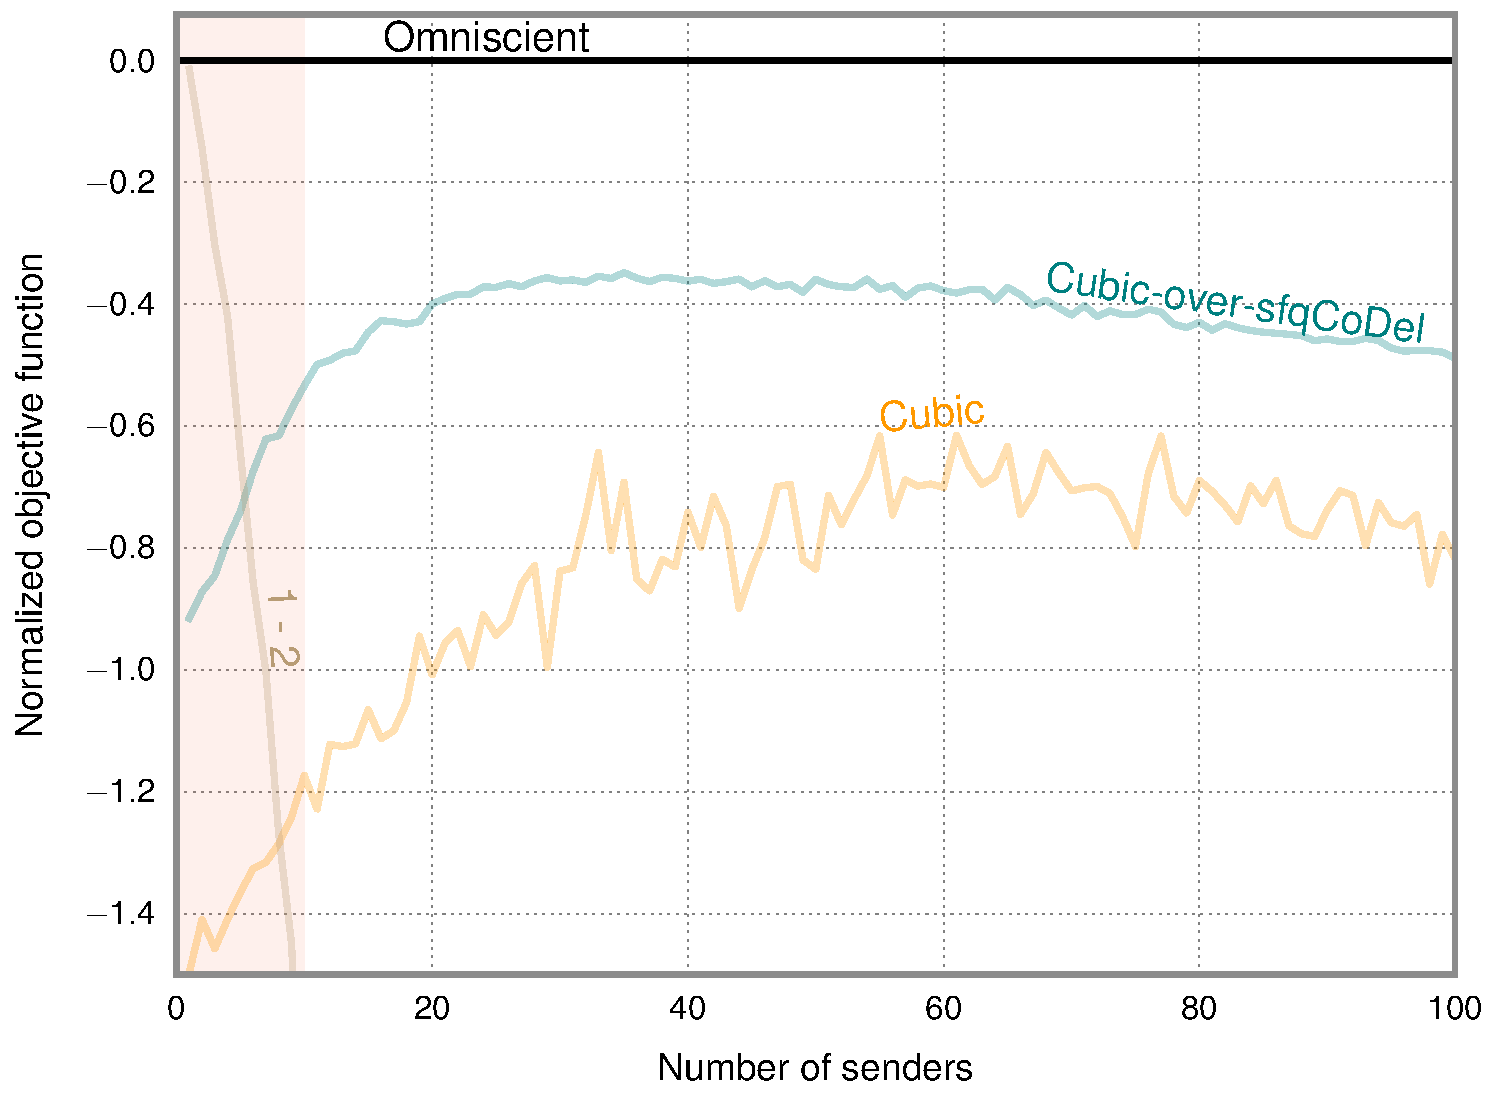
\includegraphics[width=4.1 in]{muxing-span-Tao-1-10.pdf}}\only<6>{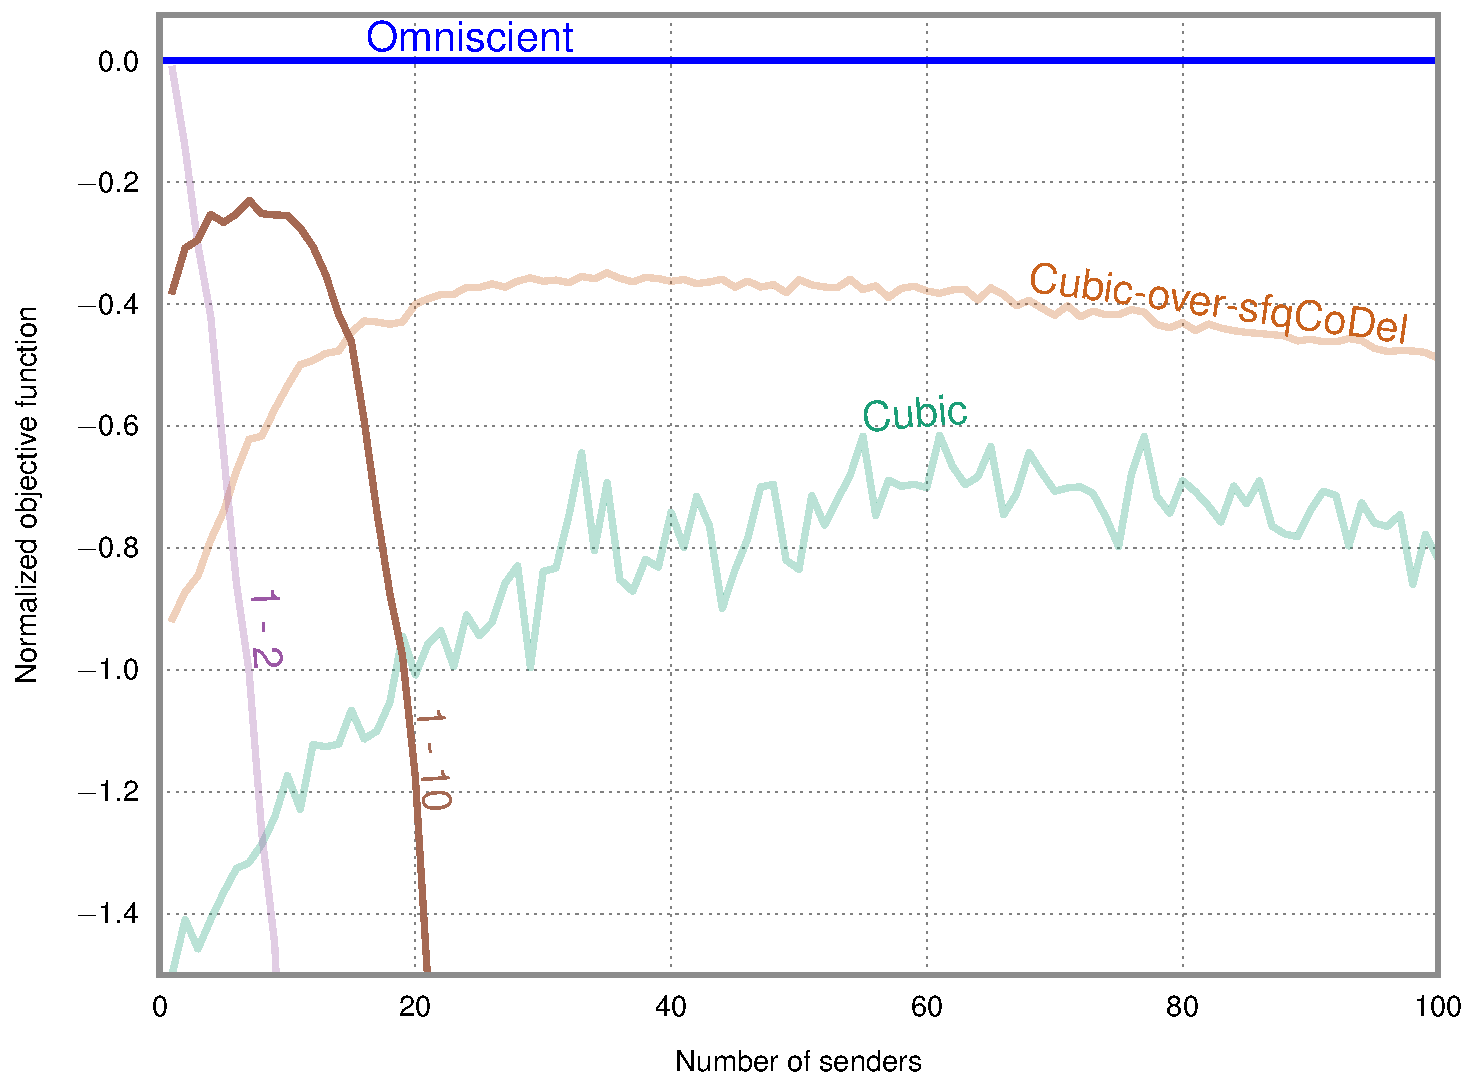
\includegraphics[width=4.1 in]{muxing-Tao-1-10.pdf}}\only<7>{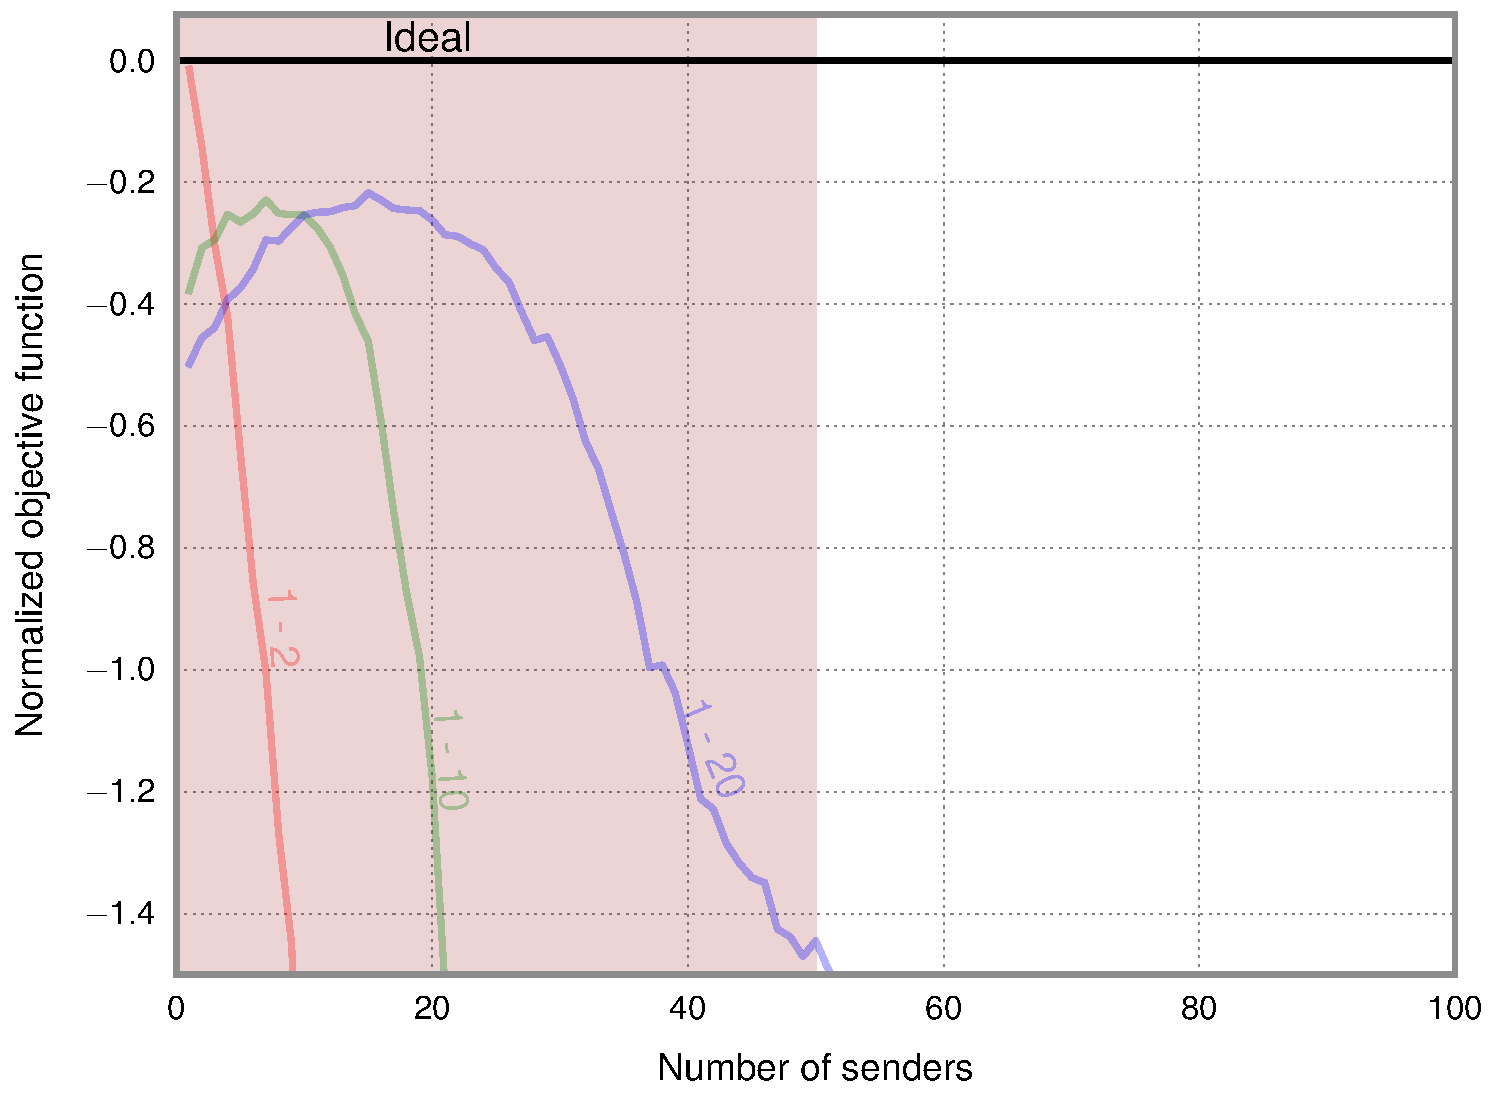
\includegraphics[width=4.1 in]{muxing-span-Tao-1-50.pdf}}\only<8>{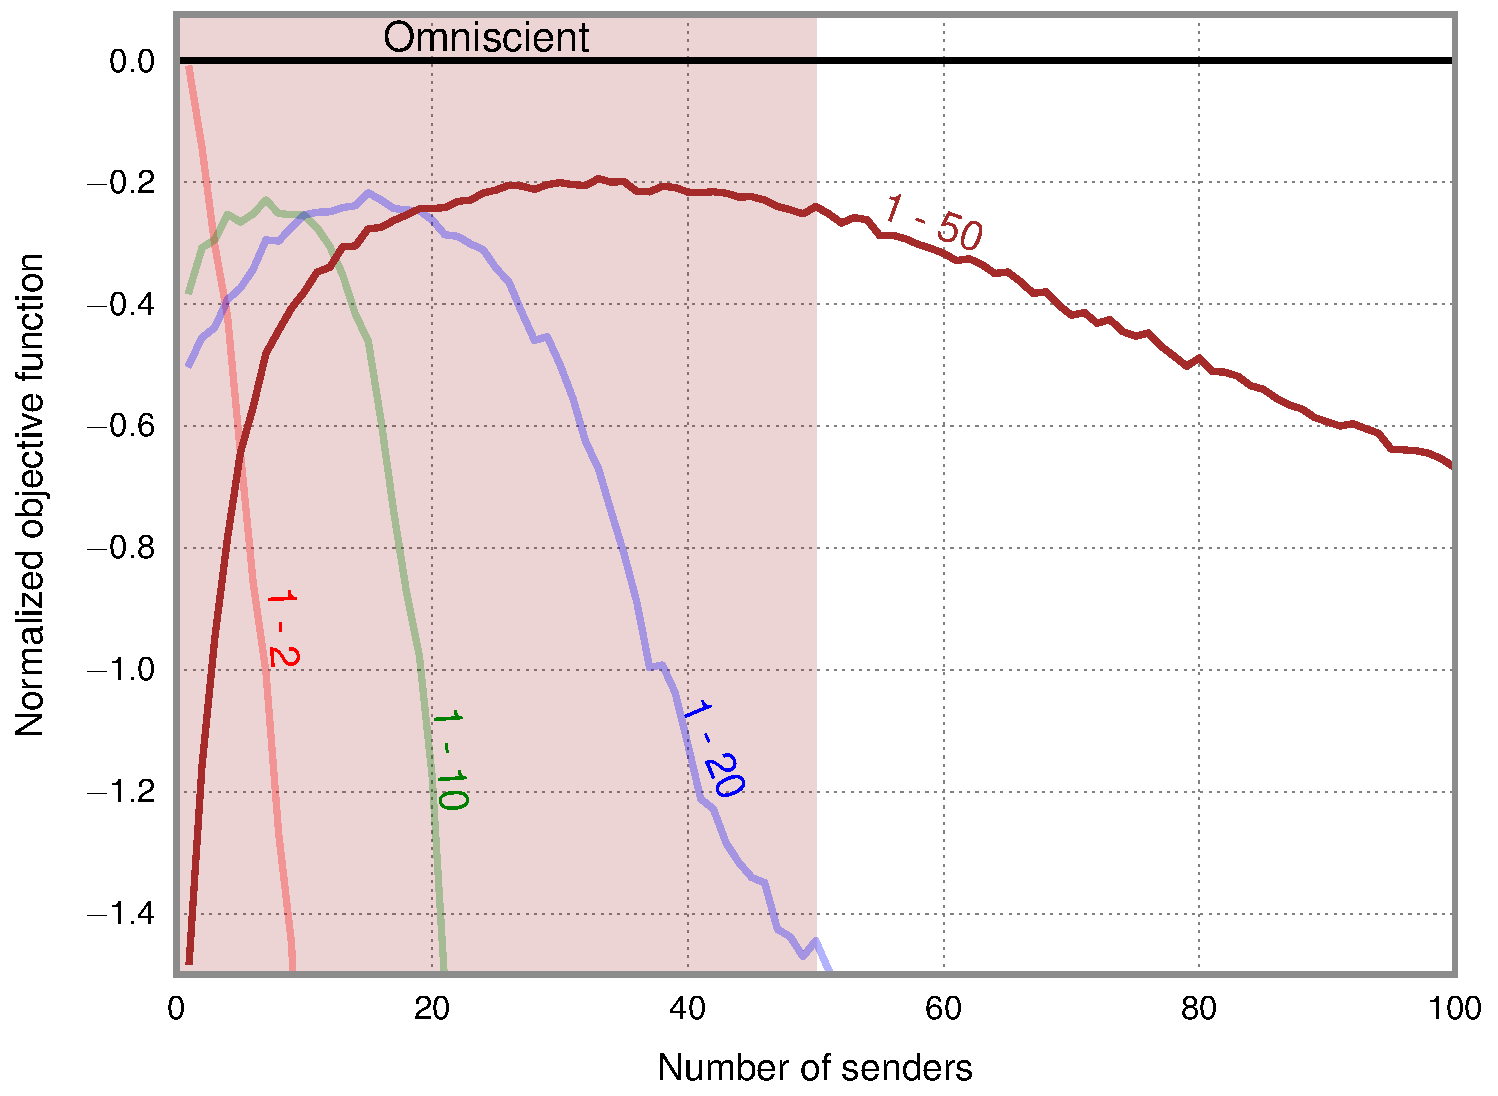
\includegraphics[width=4.1 in]{muxing-Tao-1-50.pdf}}\only<9>{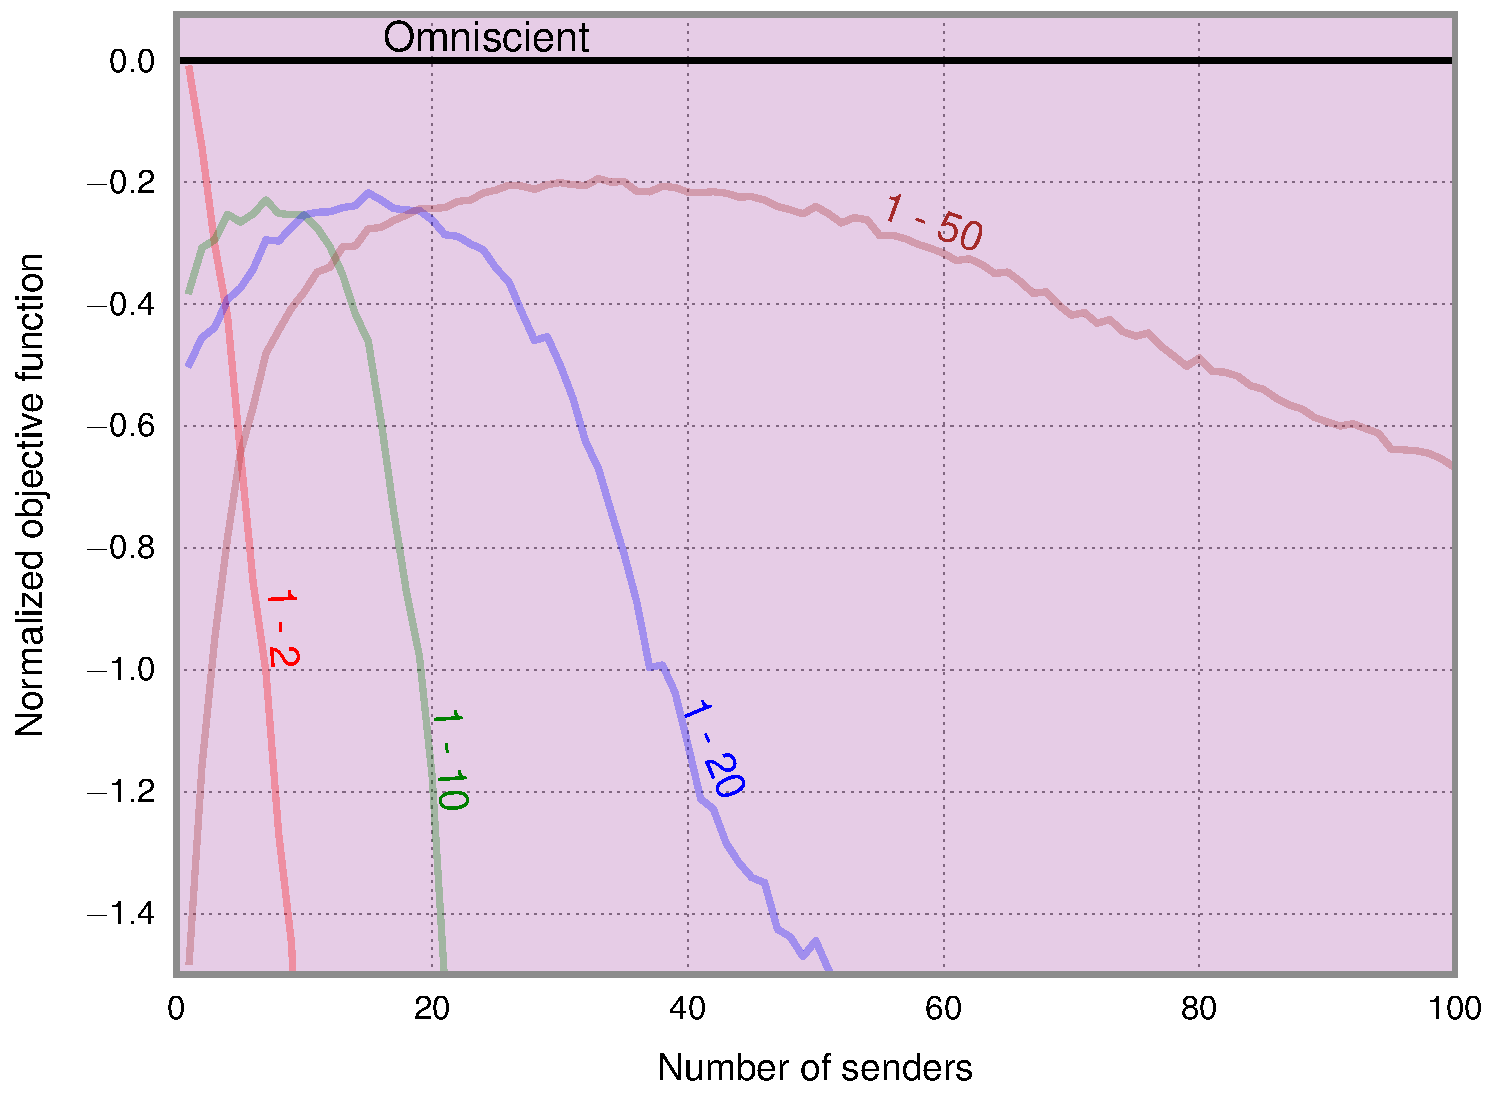
\includegraphics[width=4.1 in]{muxing-span-Tao-1-100.pdf}}\only<10>{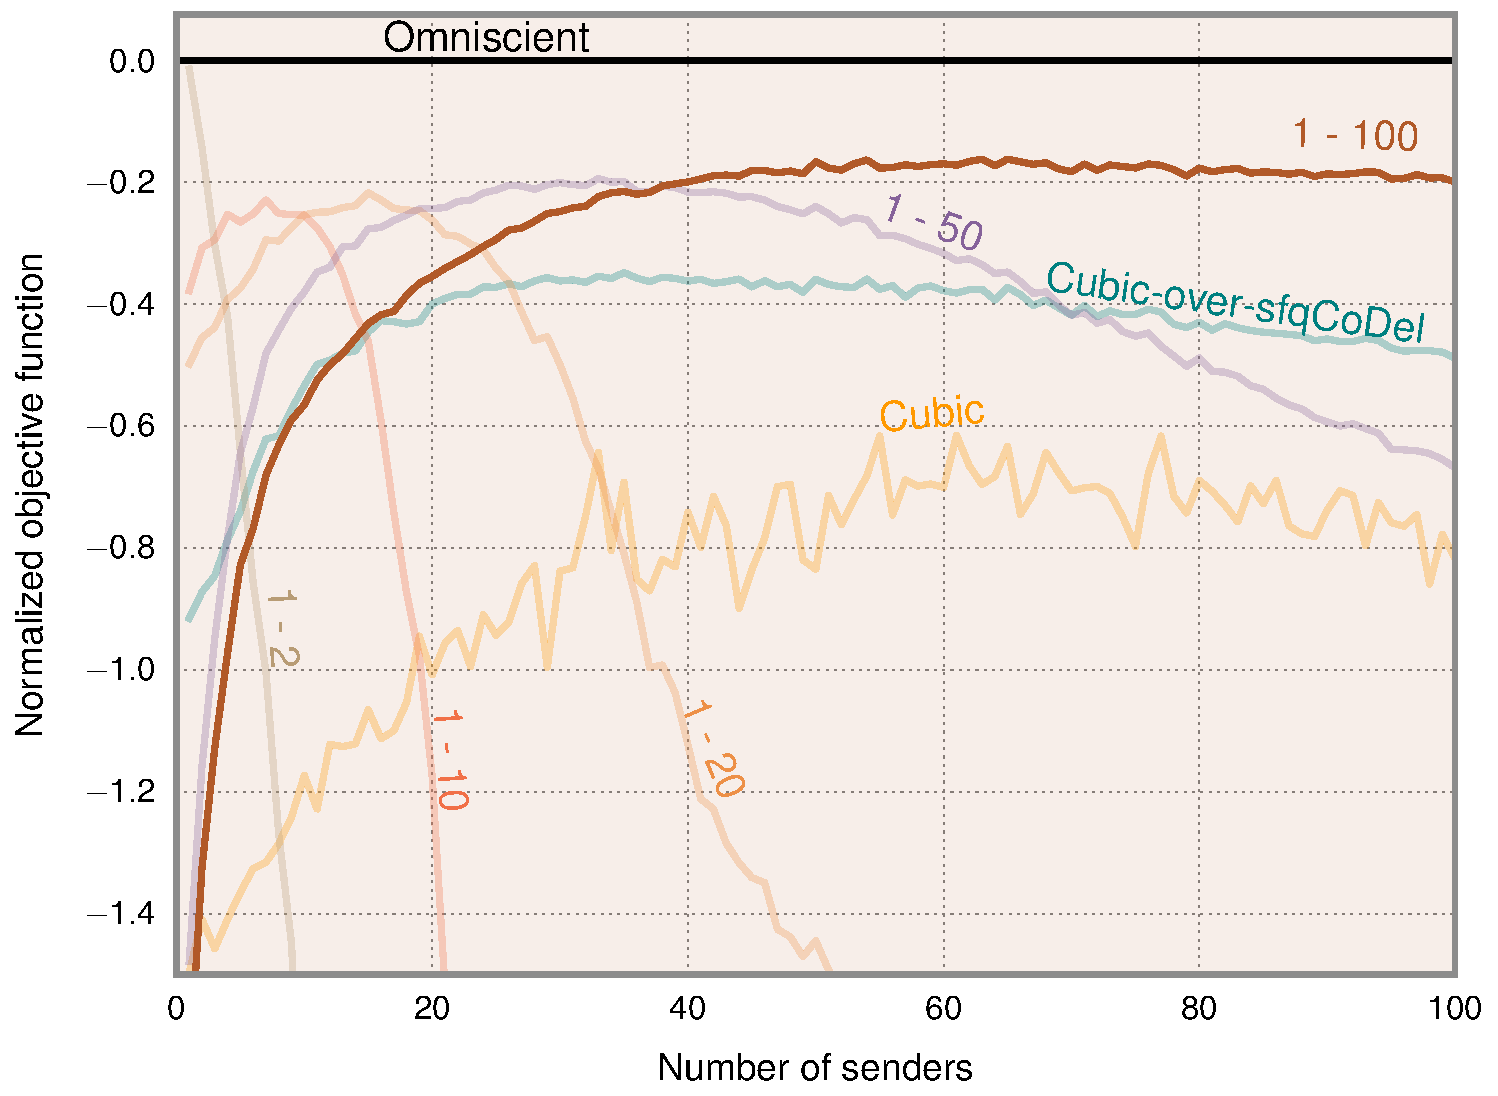
\includegraphics[width=4.1 in]{muxing-Tao-1-100.pdf}}\only<11>{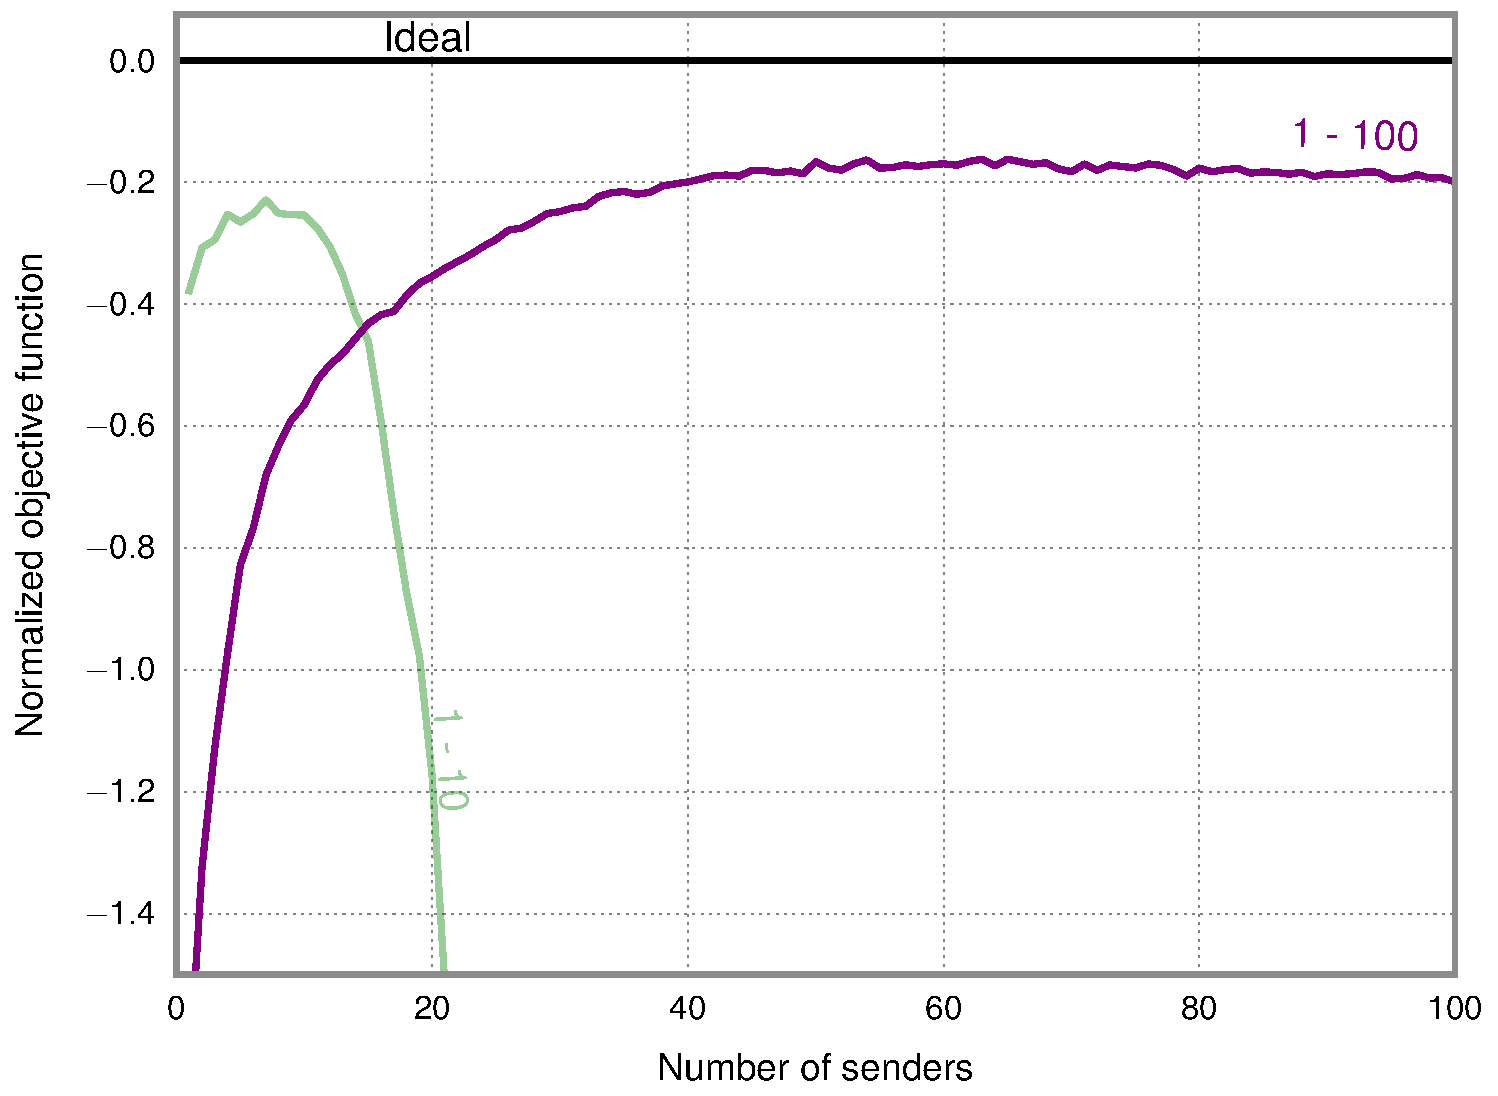
\includegraphics[width=4.1 in]{muxing-100-and-10-only.pdf}}\only<12>{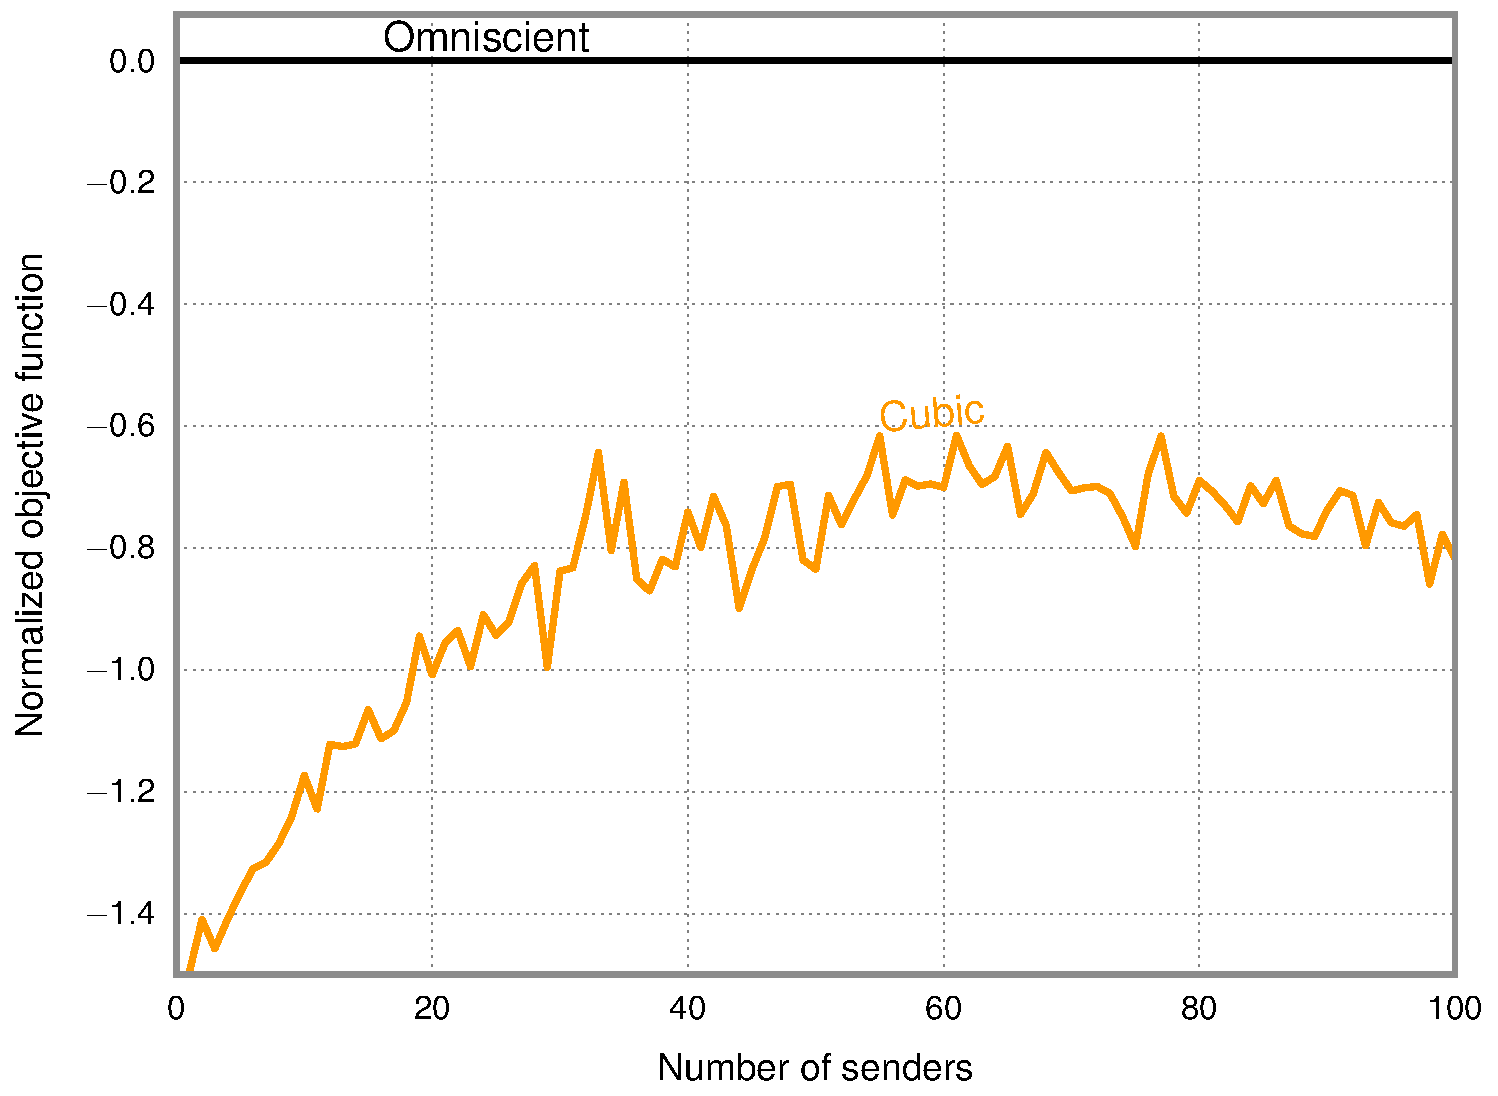
\includegraphics[width=4.1 in]{muxing-Cubic.pdf}}\only<13>{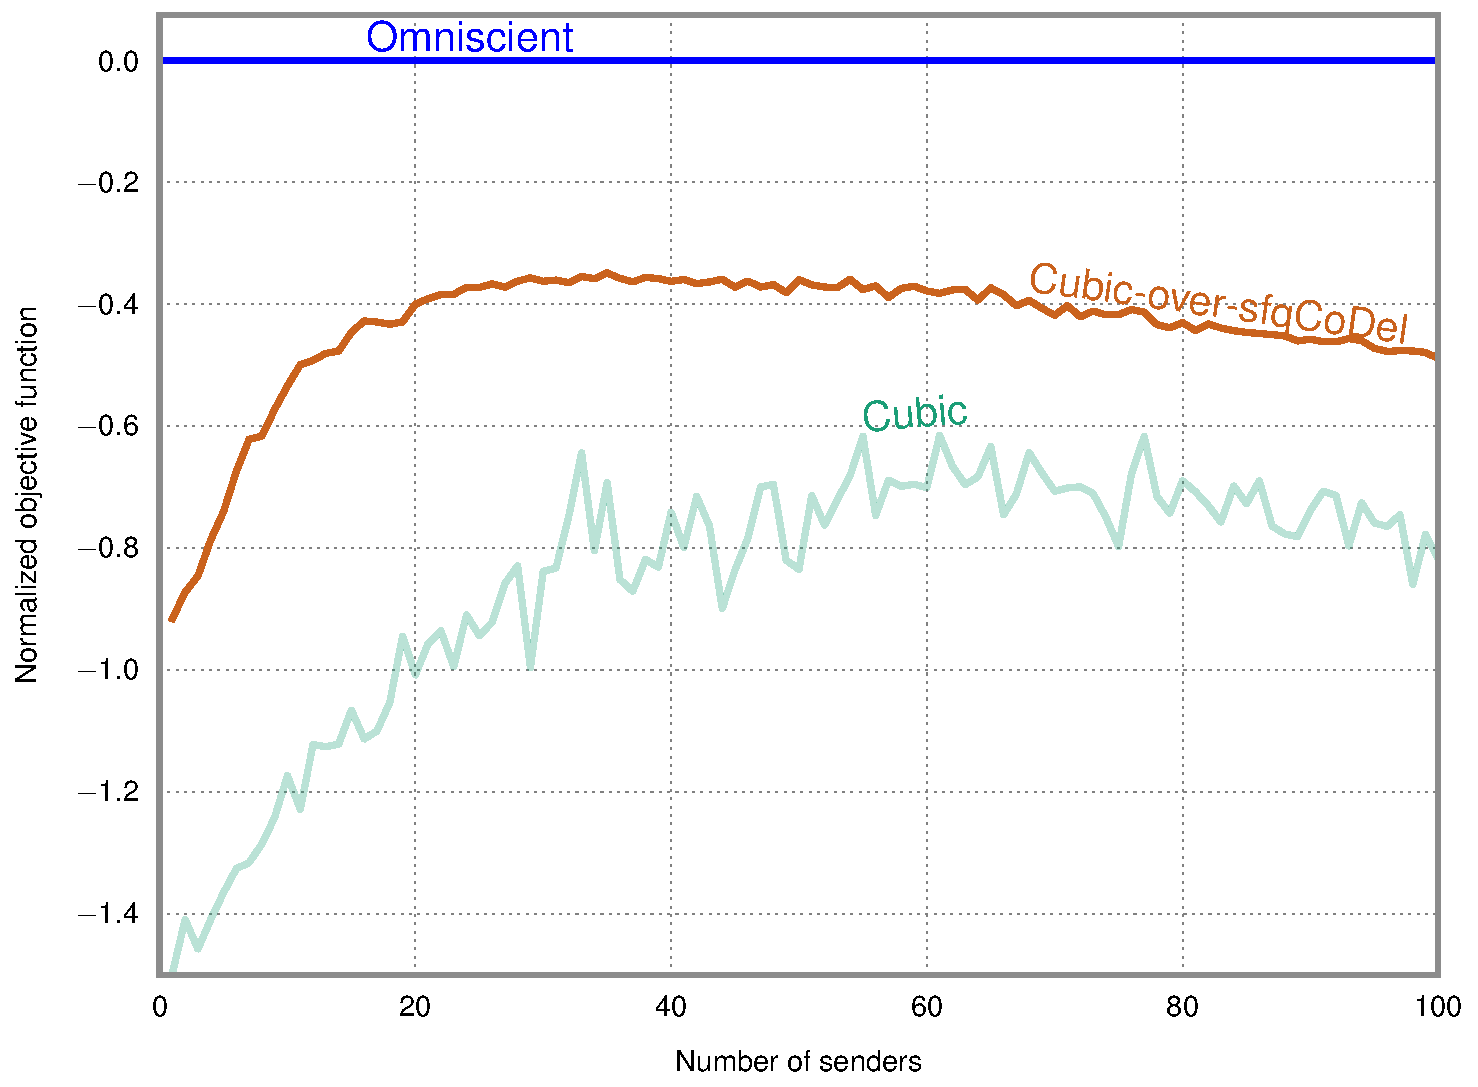
\includegraphics[width=4.1 in]{muxing-Cubic-over-sfqCoDel.pdf}}\only<14>{Tradeoff between performance with few senders and performance with many senders}

\end{centering}
\end{frame}
